\documentclass[10pt,a4paper,twocolumn]{article}
\usepackage[margin=18mm,columnsep=7mm]{geometry}
\usepackage{amsmath,amssymb,graphicx,booktabs,microtype}
\usepackage[numbers,sort&compress]{natbib}
\usepackage{lineno}
\usepackage{fancyhdr}
\usepackage[colorlinks=true,allcolors=blue]{hyperref}
\hypersetup{pdftitle={Separating arrival rounding, source startup, and reverberation in three-microphone azimuth estimation},pdfauthor={Aneesh Arnav Chikkala},pdfsubject={Preprint for author review; not peer reviewed}}
\usepackage{caption}
\usepackage{flushend}
\captionsetup{font=small,labelfont=bf}
\graphicspath{{../figures/}}
\setlength{\parindent}{1em}
\setlength{\parskip}{0pt}
\setlength{\textfloatsep}{12pt}
\pagestyle{fancy}\fancyhf{}
\fancyhead[L]{\scriptsize Three-microphone azimuth estimation}
\fancyhead[R]{\scriptsize Preprint for author review}
\fancyfoot[C]{\small\thepage}
\renewcommand{\headrulewidth}{0.3pt}
\title{Separating arrival rounding, source startup, and reverberation\linebreak in three-microphone azimuth estimation}
\author{Aneesh Arnav Chikkala}
\date{8 September 2026\\\small Preprint, version 1 for author review. Not peer reviewed.}
\begin{document}
\twocolumn[\maketitle
\begin{abstract}
\noindent\textbf{Purpose.} Small-array simulations can mix propagation discretization, source history, and acoustic effects. We quantify these contributions for a fixed three-microphone azimuth estimator.
\textbf{Methods.} Independent analytical and image-source references verify a fractional-delay shoebox model. A frozen campaign contains 276,480 GCC-PHAT frame evaluations, paired rounding/startup/reflection controls, and independent records for averaging. Uncertainty resamples whole recordings within fixed scenes.
\textbf{Results.} Final numerical refinements change checked estimates by less than $0.026^\circ$. At 10 dB direct-referenced SNR, direct-path RMSE increases from $0.923^\circ$ to $2.300^\circ$ after arrival rounding. In the high-reverberation subset, first-frame RMSE is $4.16^\circ$ at source onset versus $42.51^\circ$ with populated prehistory. Averaging 128 frames reduces held-out RMSE from $1.60^\circ$ to $0.84^\circ$ in the low subset and from $39.04^\circ$ to $10.16^\circ$ in the high subset. A geometry-only timing bound accounts for shared-microphone dependence.
\textbf{Conclusion.} Source history can create a large apparent accuracy benefit; arrival rounding introduces a separate, measurable distortion. Residual errors depend on the chosen acoustic scenes and estimator. These computations establish neither a universal reverberation floor nor hardware performance.
\end{abstract}
\par\vspace{3mm}
\noindent\textbf{Keywords:} acoustic localization; GCC-PHAT; image-source method; numerical verification; source history; \mbox{uncertainty}
\vspace{5mm}]
\linenumbers

\section{Introduction}
Estimating source direction from a compact microphone array appears to be a simple delay problem. The simulation used to evaluate it is less simple: it must construct microphone signals, represent fractional propagation times, choose an observation interval, estimate delays, and interpret them through an array model. An error introduced at any one of these steps may be attributed incorrectly to room acoustics. This is especially consequential when the acoustic travel time across the array spans only a small number of samples.

Generalized correlation is an established approach to time-delay estimation \citep{knapp}. Equilateral three-microphone arrays combined with GCC-PHAT have already been studied experimentally and numerically \citep{catur}. Fractional-delay filtering is also established \citep{laakso}. The present work proposes neither a new estimator nor a new microphone geometry. Its purpose is to make a particular computational evaluation traceable and to test which conclusions survive numerical and recording-protocol controls.

The image-source method provides an explicit model of specular shoebox propagation \citep{allen}. It allows matched experiments that would be difficult to realize physically, such as retaining the same source and noise while removing every reflection. However, an image model still requires reflection coverage, a duration cutoff, and a representation of noninteger arrival times. A simulator can also change the problem by beginning each analysis frame with an empty room. Numerical verification and physical validation therefore answer different questions. Recent acoustic benchmarking emphasizes the distinction between implementation errors, numerical convergence, and differences in physical assumptions \citep{ernoult}.

We study three specific choices: rounding each path arrival to the sample grid, omitting source prehistory, and including reflections. Exact plane-wave and spherical controls separate algebraic recovery from finite-distance curvature. Independent room enumeration and refinement tests establish numerical resolution before a confirmatory campaign. Paired records identify changes caused by the three choices, while separate long recordings test averaging. A deterministic precision criterion relates bounded microphone-arrival errors to geometry without assuming independent pair-delay errors.

The contribution is a verified attribution and replication study with inspectable frame results, not an exhaustive survey or a claim of priority. The scope is one stationary synthetic source, ideal matched microphones, horizontal azimuth, and three prescribed room geometries. Real recordings, moving or multiple sources, hardware timing, microphone mismatch, and scattering are outside the evaluation.

\section{Physical and signal-processing model}
\subsection{Array and arrival geometry}
The three microphone positions relative to the array center are
\begin{equation}
 \mathbf m_i=R[\cos\phi_i,\sin\phi_i]^T,\quad
 \phi_i\in\{90^\circ,210^\circ,330^\circ\},
\end{equation}
with circumradius $R=0.05$ m and pair spacing $\sqrt{3}R=0.0866$ m. Sound speed is fixed at $c=343$ m/s. The source is 1.5 m from the array center, at the microphone height. The direct spherical arrival is $t_i=\|\mathbf s-\mathbf m_i\|/c$, using horizontal relative coordinates. For an ideal plane wave with unit source direction $\mathbf u$, $t_i=-\mathbf m_i^T\mathbf u/c$ up to an irrelevant common delay.

For pairs $i<j$, define $\tau_{ij}=t_i-t_j$ and let the rows of $A$ be $(\mathbf m_i-\mathbf m_j)^T$. The estimator interprets its three pair delays through
\begin{equation}
 \widetilde{\mathbf u}=-cA^+\widehat{\boldsymbol\tau},\qquad
 \widehat\theta=\operatorname{atan2}(\widetilde u_y,\widetilde u_x).
 \label{eq:solve}
\end{equation}
All pairs have equal weight. The direction vector is not constrained to unit norm before taking its angle. Thus, exact spherical arrivals can retain a finite-distance mismatch when interpreted by this planar far-field solve. This contribution is not an interpolation error.

\begin{figure*}[t]
\centering
\includegraphics[width=\textwidth]{fig1_geometry_controls.pdf}
\caption{Array and paired controls. The source-direction arrow indicates azimuth; its length is schematic, while the microphone coordinates are to scale. The source distance is 1.5 m. Each of the eight combinations shares the same underlying source and microphone-noise samples for a given scene and record. Onset means one startup at the beginning of the complete recording.}
\label{fig:geometry}
\end{figure*}

\subsection{Room responses}
Each room is a three-dimensional rectangular enclosure with six frequency-independent pressure-reflection coefficients. For room side lengths $L_a$, source coordinates $s_a$, integers $n_a\in[-K,K]$, and parities $p_a\in\{0,1\}$, the image coordinate is
\begin{equation}
 s^{\mathrm{img}}_a=2n_aL_a+(1-2p_a)s_a.
\end{equation}
The corresponding low/high wall reflection counts are $|n_a-p_a|$ and $|n_a|$. A path of length $r$ has delay $r/c$ and pressure gain $\prod_w\beta_w^{N_w}/(4\pi r)$. Paths longer than $cT_h$ are omitted. The main settings are $K=76$ and $T_h=1.2$ s. These choices are based on refinement, rather than a nominal reflection order alone.

Uniform wall absorption uses the nominal Sabine relation $\alpha=0.161V/(S T_{\mathrm{nom}})$ and $\beta=\sqrt{1-\alpha}$, where $V$ and $S$ are volume and surface area. $T_{\mathrm{nom}}$ labels an absorption setting; it is not asserted to equal the realized reverberation time. Calibration of such relationships is itself a room-model problem \citep{bellows}. Frequency-independent specular reflection is a deliberate simplification: diffraction, diffuse scattering, air attenuation, microphone directivity, and material phase responses are absent.

For fractional arrivals, each path is deposited linearly on a time grid 32 times finer than the acquisition grid. A normalized Kaiser-windowed sinc decimation filter, with shape parameter 8.6 and half-width 32 acquisition samples, then produces the response. A separate rounded condition deposits each path at $\operatorname{round}(f_s r/c)$ without that reconstruction. The same image coverage and gains are used. An explicit switch produces direct-only responses, which retain the same array/source geometry and overall response length.

\subsection{Continuous source and noise}
Sampling is at 48 kHz. The source is a Gaussian sequence projected by an FFT mask onto 300--3400 Hz and normalized in RMS. Each record includes 59,682 samples of source prehistory before the analysis interval. Convolution uses the full response. All microphone signals then pass through the same causal Butterworth bandpass with prototype order four (four second-order sections, total order eight) at 300--3400 Hz. The noise channels originate from independent Gaussian sequences filtered through the same acquisition response.

Noise power is calibrated using the acquired, steady, direct-only signal averaged across the three microphones and the full analysis interval. The specified SNR is the ratio of this reference power to the acquired noise power. Adding reflections therefore does not change the noise realization or its scaling within a paired comparison. This SNR should not be interpreted as the ratio of the complete reverberant signal power to noise power.

Steady records retain the source prehistory. Onset records use exactly the same source samples inside the analysis interval but zero the preceding source samples once. Both retain the same noise. Switching the source also introduces an onset spectrum; the experiment includes that physical transient. The primary analysis uses contiguous, nonoverlapping 2048-sample frames, each 42.667 ms long. A separately labeled exploratory diagnostic resets the source and acquisition history for every frame; it is not treated as a continuous recording.

\subsection{GCC-PHAT implementation}
Each microphone frame is mean-centered and multiplied by a symmetric Hann window. The transform size is the next FFT-efficient size at least twice the frame length, here 4096. With $G_{ij}[k]=X_i[k]X_j^*[k]$, the regularized cross spectrum is
\begin{equation}
 W_{ij}[k]=\frac{G_{ij}[k]}{\max\{|G_{ij}[k]|,\,10^{-3}\max_l|G_{ij}[l]|+10^{-12}\}},
\end{equation}
and is zeroed outside 300--3400 Hz. The regularization maximum is computed before band exclusion. The inverse transform is evaluated at eightfold correlation sampling. Only candidate lags within $\|\mathbf m_i-\mathbf m_j\|/c$ are searched. A three-point quadratic peak refinement is clipped to one correlation-grid step and then to the physical delay bound. Equation~\ref{eq:solve} converts the three refined delays to azimuth. These implementation choices define the method evaluated here; ``GCC-PHAT'' alone would not specify them.

\subsection{Acoustic descriptors}
Acquired impulse responses produce the reverse-integrated squared response, following the energy-decay approach \citep{schroeder}. We fit T20 over $-5$ to $-25$ dB and extrapolate the fitted slope to 60 dB; EDT, T30, and fit quality are retained as supplementary outputs. Energy is summed across microphones before decay fitting. A component direct-to-reverberant ratio is computed from the energies of the separately filtered direct and reflected responses. Their coherent cross term is also retained. This ratio does not presume that direct and reflected energy add without interference. Direct and all six first-order reflection times and gains accompany each scene.

\section{Verification and experimental design}
\subsection{Independent controls and numerical tolerance}
An independent scalar implementation solves the two-by-two normal equations without importing the production geometry solve. Plane-wave recovery, spherical propagation, cardinal directions, and all six channel permutations are checked. The analytical sweep spans 720 angles, radii 0.025/0.05/0.10 m, source distances 0.5/1.5/5/20 m, and rates 16/48/96/192 kHz: 34,560 conditions. A separate harmonic oracle compares directly evaluated continuous-time signals with fractional-delay FIR signals at matched physical bandwidth, duration, and observation time.

The room reference enumerates reflected tiles through a different integer/parity construction and evaluates each path with its exact frequency-domain phase. It imports neither the production image enumeration nor the fractional response builder. Tests compare path counts, spectra, and resulting angle estimates, including unequal wall coefficients. Image extent is refined until two successive changes are below $0.05^\circ$ in angle, 1\% in T20, and 0.1\% in probe spectrum. Response duration is checked separately at fixed extent. Initial oversampling checks compared factors 8, 16, and 32 with the independent reference. The final factor 32 is checked against a full-extent independent image sum and refined to 64 on stochastic records.

The $0.05^\circ$ discrepancy target is chosen for interpreting effects of roughly $0.5^\circ$ or larger. It is not an acoustic accuracy requirement. Refinement on stochastic recordings is also necessary because a small response change could alter selection between nearly tied peaks. Exploratory pilot inputs and confirmatory inputs have separate identity-derived random streams. Numerical exceptions are retained rather than silently removed.

\subsection{Frozen campaign}
Table~\ref{tab:protocol} summarizes the protocol, frozen before confirmatory results were generated. The rooms are $6\times5\times3$, $5\times4\times2.8$, and $8\times6\times3.2$ m. Array centers are at room-coordinate fractions $(0.5,0.5,0.5)$ and $(0.6,0.45,0.5)$. Nominal decay settings are 0.15, 0.30, and 0.60 s. Directions are $7.37^\circ+30^\circ j$, $j=0,\ldots,11$. All coordinates are inside the rooms, with minimum source/microphone wall clearance 0.312 m.

The paired and long-record subset uses six acoustic states: the centered, nominal-0.15-s state and the offset, nominal-0.60-s state in each room. Including 12 directions gives 72 physical scenes. We call these the low and high subsets, respectively. Placement and absorption differ between them; their difference is not a controlled single-factor RT comparison. The core matrix, in contrast, includes both placements at every nominal decay setting.

\begin{table}[t]
\centering\small
\caption{Frozen confirmatory allocation. A frame is 2048 samples. Counts exclude exploratory and numerical-reference work.}
\label{tab:protocol}
\begin{tabular}{@{}lrr@{}}\toprule
Study & Scenes & Evaluations\\\midrule
Core: 3 SNRs, $5\times32$ frames & 216 & 103,680\\
Attribution: 7 additional variants & 72 & 80,640\\
Long records: $10\times128$ frames & 72 & 92,160\\\midrule
Primary total & & 276,480\\\bottomrule
\end{tabular}
\end{table}

The eight attribution variants cross fractional/rounded arrivals, steady/onset history, and direct/reflected propagation (Fig.~\ref{fig:geometry}). At 10 dB, five 32-frame records are shared across all eight conditions. The corrected fractional/steady/reflected condition is reused exactly from the core matrix. In each of the 72 long-record scenes, five new 128-frame recordings estimate bias/covariance and five different recordings test averaging. These streams do not overlap with pilot or core records.

The fixed secondary subset contains 24 scenes: four directions in each of the six states. Five 32-frame records at 10 dB assess a $17^\circ$ array rotation, a non-equilateral triangle, unequal wall absorption, and a 300--1700 Hz source band. The estimator and acquisition band remain 300--3400 Hz in the latter test. Variations use separate random namespaces and are scope probes rather than paired causal contrasts with the original geometry. Baseline SRP-PHAT uses the same input frames, band, window, and regularization, but sums pair cross spectra at continuous predicted plane-wave delays over azimuth. A $0.25^\circ$ angular grid with quadratic refinement is checked against a $0.05^\circ$ grid. Reverberant localization has a long-established algorithmic literature \citep{dibiase}; this is a limited matched comparison, not an estimator ranking across applications.

\subsection{Errors and uncertainty}
Signed error is wrapped to $[-180^\circ,180^\circ)$. We report RMSE, median and 90th-percentile absolute error, circular bias, and the proportion exceeding $5^\circ$. The latter is a predeclared descriptive threshold, not a perceptual or device-acceptance standard. Error tails and difficult scenes remain in every aggregate.

We use 2000 bootstrap draws \citep{efron}, resampling whole recordings with replacement within each fixed scene. Paired variants use the same selected records. Thus the intervals describe source/noise variability conditional on the selected geometries and directions. Three room geometries do not support a population-of-rooms uncertainty statement. Individual scene summaries accompany balanced pooled estimates, and the 160 frames in a short-record scene are not counted as 160 independent experimental replicates.

Attribution contrasts use paired signed errors and paired squared errors. We do not subtract RMSE values to manufacture additive error components. Factorial main effects average over the other two factors; interactions use the corresponding differences of differences. Signed wrapped means are descriptive and can conceal multimodal or opposing errors, so squared-error contrasts and the complete distributions remain central.

\subsection{Held-out averaging}
For $n=1,2,4,8,16,32,64,128$, direction estimates are averaged circularly over contiguous nonoverlapping blocks. The longest duration is 5.461 s. A small-error model predicts
\begin{equation}
 \operatorname{MSE}(\overline e_n)\simeq b^2+
 \frac{1}{n}\left[\gamma_0+2\sum_{\ell=1}^{n-1}
 \left(1-\frac{\ell}{n}\right)\gamma_\ell\right].
 \label{eq:variance}
\end{equation}
Training records provide circular bias $b$ and record-centered autocovariance estimates. Covariances are truncated at lag 32 and Bartlett-tapered; negative predicted variances are clipped to zero. A separate independent-frame approximation sets nonzero lags to zero. Predictions receive substantive interpretation only for scenes satisfying the frozen training rule: circular resultant at least 0.95 and absolute circular mean error at most $15^\circ$. All scenes retain empirical held-out results. The rule is a concentration screen, not proof that rare errors or nonstationarity are absent.

\section{Results}
\subsection{Verification and realized decay}
Table~\ref{tab:verification} summarizes the final checks. The exact plane-wave solve agrees to $5.7\times10^{-14}$ degrees, and the independent scalar reference differs by at most $7.3\times10^{-12}$ degrees. At the selected direct-path FIR half-width 32, the largest oracle/FIR angular discrepancy is $3.7\times10^{-5}$ degrees. Increasing GCC correlation sampling from 8 to 64 changes direct-path estimates by at most $0.000495^\circ$.

At the final selected image coverage, the independent room check compares approximately 5.22 million paths per microphone. Relative spectral discrepancy is $1.13\times10^{-5}$ and angle discrepancy is $0.000807^\circ$. Coarse image coverage changed one high-setting estimate by more than $100^\circ$ before convergence. A coarse fractional grid also missed the spectral target; both findings are documented in the numerical notes. They motivated refinement, not relaxation of the tolerance.

A stronger internal-review check extended duration and image support together. The initial 0.9-s/extent-48 campaign failed this check: ten of 960 frames exceeded $0.05^\circ$, with a maximum change of $0.16551^\circ$. That campaign was preserved and superseded. The final 1.2-s/extent-76 model, with propagation factor 32, passes a joint extension to 1.5 s/extent 96 with maximum change $0.01273^\circ$. The same scientific matrix and analysis rules were then rerun with new source/noise identities. Final results below contain only this revised campaign; the supplement records the correction.

\begin{table}[t]\centering\small
\caption{Final numerical verification. Values are maximum angular discrepancies in the stated checks, not errors against source azimuth.}
\label{tab:verification}
\begin{tabular}{@{}lr@{}}\toprule
Check & Change (deg)\\\midrule
Full room reference & 0.000807\\
Joint duration/domain & 0.012726\\
Propagation grid 32 to 64 & 0.006965\\
Image extent 76 to 84 & 0.000000\\
GCC factor 8 to 16 & 0.025930\\
SRP angular grid refinement & 0.002310\\
\bottomrule\end{tabular}\end{table}



On the confirmatory secondary subset, increasing propagation oversampling from 32 to 64 changes individual estimates by at most $0.006965^\circ$; image extent 76 to 84 changes them by $0^\circ$; GCC factor 8 to 16 changes them by $0.02593^\circ$. SRP grid refinement changes estimates by at most $0.002311^\circ$. No checked stochastic frame exceeds $0.05^\circ$ (Fig.~\ref{fig:numerics}). These selected checks do not constitute a worst-case theorem for every possible stochastic input.

\begin{figure*}[t]
\centering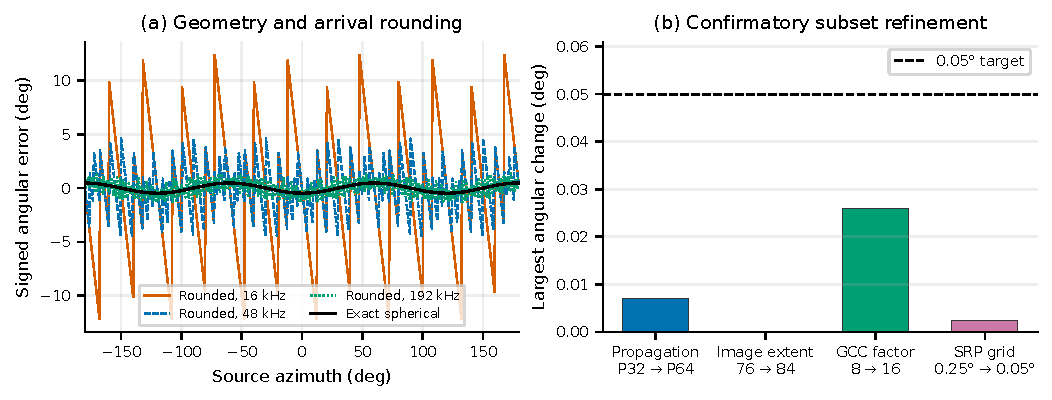
\includegraphics[width=\textwidth]{fig2_numerical_verification.pdf}
\caption{Numerical effects and checks. (a) Analytical arrival rounding at $R=0.05$ m and source distance 1.5 m; exact spherical arrivals are interpreted by the same far-field solve. These are not noisy waveform-estimation results. (b) Maximum individual angular changes over the fixed 24-scene confirmatory subset, five records and 32 frames per scene. The dashed line is a numerical-discrepancy target.}
\label{fig:numerics}
\end{figure*}

Realized band T20 ranges are 0.083--0.110 s, 0.259--0.295 s, and 0.586--0.683 s for nominal settings 0.15, 0.30, and 0.60 s, respectively. Minimum T20 fit $R^2$ is 0.928 in the low setting and 0.994 in the other settings. A nominal RT label therefore cannot replace response measurement. Component DRR spans approximately $+9.53$ to $-10.77$ dB across the full matrix.

\subsection{Corrected room performance}
At 10 dB, the corrected core RMSE is $1.620^\circ$ [95\% interval 1.599, 1.641] for nominal 0.15 s, $11.954^\circ$ [11.168, 12.771] for 0.30 s, and $37.233^\circ$ [36.359, 38.111] for 0.60 s. The proportions above $5^\circ$ are 0.86\%, 27.38\%, and 62.30\%. The corresponding 20-dB RMSEs are 1.362, 11.796, and $37.067^\circ$: reducing additive noise does not eliminate reflected-field errors in this model.

Figure~\ref{fig:core} preserves differences across rooms. At 10 dB, individual scene RMSE ranges from 0.92 to $3.16^\circ$ in the lowest setting, 2.08 to $49.08^\circ$ in the middle setting, and 6.56 to $86.16^\circ$ in the highest. These ranges are much wider than uncertainty intervals on pooled conditional means. Direction, placement, and room geometry are therefore material parts of the reported result.

\begin{figure*}[t]
\centering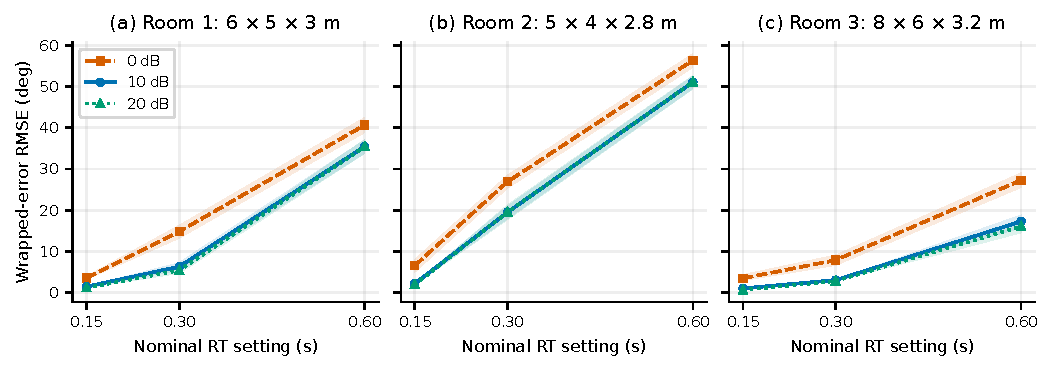
\includegraphics[width=\textwidth]{fig3_core_rooms.pdf}
\caption{Corrected fractional/steady/reflected core results, with rooms shown separately. Each point pools two placements, 12 directions and five 32-frame records. Bands are 95\% bootstrap intervals conditional on those fixed scenes. The horizontal coordinate is the nominal absorption/RT setting, not an assertion of realized RT.}
\label{fig:core}
\end{figure*}

\subsection{Paired rounding and source-history effects}
Table~\ref{tab:effects} summarizes the paired squared-error contrasts. Across the 72 attribution scenes at 10 dB, steady direct-path RMSE is $0.923^\circ$ [0.912, 0.934] with fractional arrivals and $2.300^\circ$ [2.287, 2.313] with rounding. The paired increase in mean squared error is 4.438 deg$^2$ [4.380, 4.493]. This establishes a rounding effect after waveform processing, separately from the analytical geometry diagnostic.

With reflections, steady RMSE is $27.365^\circ$ for fractional arrivals and $28.112^\circ$ after rounding. The paired squared-error increase is 41.448 deg$^2$ [11.974, 70.571]. Its magnitude and uncertainty differ markedly from the direct-path contrast. This pooled penalty does not establish an identical effect in every scene: rounding changes coherent interference and can alter which peak is selected.

The source-history contrast is strongest immediately after startup (Fig.~\ref{fig:paired}). In the high subset, the first-frame RMSE is $4.157^\circ$ at onset versus $42.508^\circ$ with populated prehistory. By the last frame of the 1.365-s short record, both reach $41.526^\circ$ for the matched realizations. For fractional reflected signals pooled across all 72 scenes and 32 frames, onset reduces mean squared error by 42.798 deg$^2$ [22.983, 62.404], expressed as a reduction; onset-minus-steady is negative. This describes transient observation, not an improvement to the estimator.

The factorial onset-by-reflection interaction is $-49.046$ deg$^2$ [$-65.574$, $-32.891$]. The rounding-by-reflection interaction is positive, 30.762 deg$^2$ [4.770, 57.791]. Interactions and broad error tails make an independent additive error budget inappropriate. The separate exploratory per-frame-reset diagnostic gives much lower reflected RMSE than continuous records, but it uses pilot directions and is not substituted for the confirmatory time trajectory.

\begin{table}[t]\centering\footnotesize
\caption{Paired changes in mean squared error (deg$^2$), all 72 attribution scenes. Intervals resample complete records within each fixed scene.}
\label{tab:effects}
\begin{tabular}{@{}lrr@{}}\toprule
Contrast & Change & 95\% interval\\\midrule
Rounding, direct & 4.44 & [4.38, 4.49]\\
Rounding, reflected & 41.45 & [11.97, 70.57]\\
Onset, reflected & -42.80 & [-62.40, -22.98]\\
Reflections, fractional & 747.97 & [699.52, 799.81]\\
\bottomrule\end{tabular}\end{table}


\begin{figure*}[t]
\centering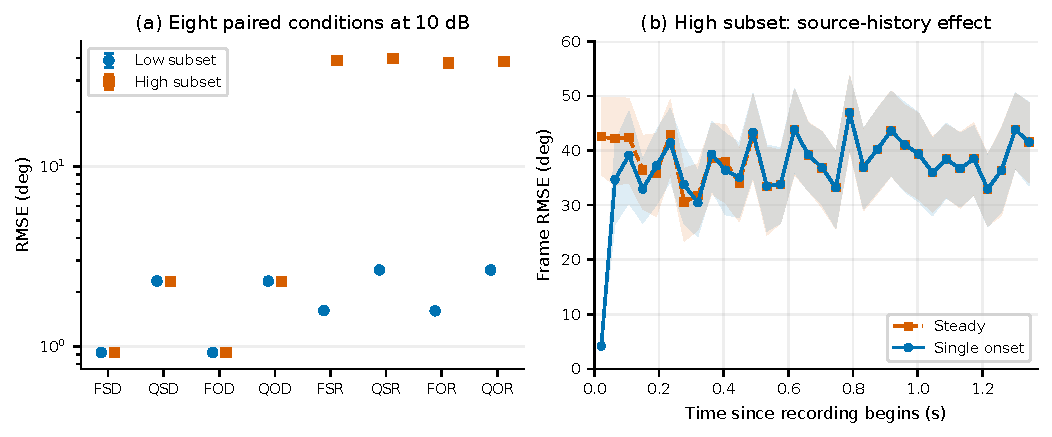
\includegraphics[width=\textwidth]{fig4_paired_attribution.pdf}
\caption{Paired attribution at 10 dB. (a) Eight combinations: F/Q, fractional/rounded; S/O, steady/onset; D/R, direct/reflected. Low and high subsets each contain 36 scenes; their placement and absorption settings differ. Error bars are record-bootstrap intervals. (b) Matched fractional reflected recordings in the high subset. The reflected field is still building in the first onset frame; later frames approach the steady condition. Time is measured from the beginning of the analyzed recording, and markers show frame midpoints.}
\label{fig:paired}
\end{figure*}

\subsection{Independent-record averaging}
Held-out results confirm a reduction in dispersion with longer averaging, without a common residual accuracy across scenes (Fig.~\ref{fig:averaging}). In the low subset, RMSE changes from $1.597^\circ$ [1.584, 1.610] for one frame to $0.835^\circ$ [0.815, 0.854] for 128 frames. In the high subset, it changes from $39.044^\circ$ [38.439, 39.607] to $10.158^\circ$ [9.404, 10.995]. At 128 frames, 46.11\% of high-subset block estimates still exceed $5^\circ$.

Forty-nine of 72 scenes pass the training concentration rule. Their held-out 128-frame RMSE is $2.013^\circ$ [1.932, 2.090], compared with $2.075^\circ$ from the bias/covariance approximation and $2.106^\circ$ from the independent-frame approximation. The long-duration aggregate is compatible with the model on the selected set, while departures at shorter durations remain visible; the tiny difference between the two approximations does not establish a useful superiority of covariance correction. The empirical results for the excluded, less concentrated scenes remain in panel (a) and the supplement. A 5.46-s observation is finite: it does not establish an asymptotic or universal reverberation floor.

\begin{figure*}[t]
\centering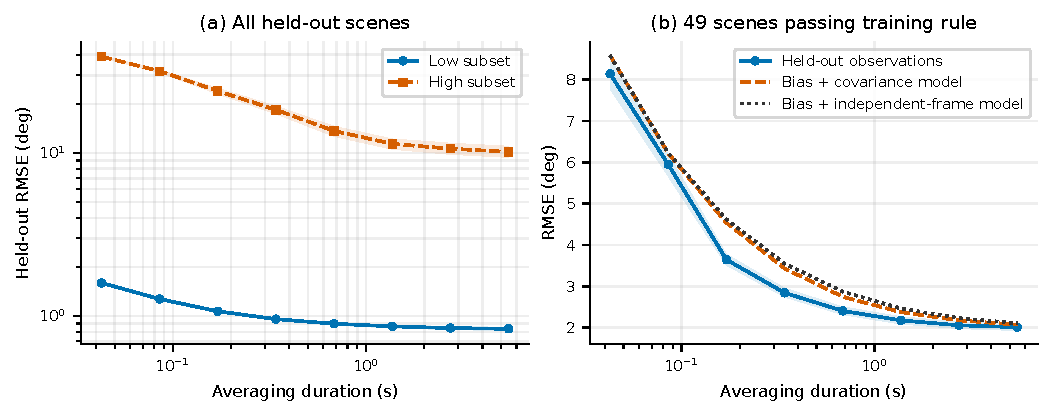
\includegraphics[width=\textwidth]{fig5_heldout_averaging.pdf}
\caption{Averaging on independent held-out recordings. (a) Circular block means in all 72 scenes, separated into low and high subsets. (b) Only the 49 scenes passing the rule determined from separate training records. Predictions are model outputs, not confidence intervals. Shaded intervals resample whole held-out recordings within each fixed scene.}
\label{fig:averaging}
\end{figure*}

\subsection{Precision criterion and scope probes}
Let $B$ be the pair-incidence matrix, so $A=BM$. Perturbing microphone arrivals by $\boldsymbol\epsilon$ changes the solved direction vector exactly by
\begin{equation}
 \delta\widetilde{\mathbf u}=J\boldsymbol\epsilon,\qquad J=-cA^+B.
\end{equation}
This retains dependence between pairs sharing a microphone. For $|\epsilon_i|\leq h$, compute $\rho=\max_{\epsilon_i\in\{-h,h\}}\|J\boldsymbol\epsilon\|$. If $\rho<\|\widetilde{\mathbf u}\|$, the exact angular extreme is attained at a vertex of the transformed box, and a simpler conservative bound is
\begin{equation}
 |\delta\theta|\leq\arcsin\frac{\rho}{\|\widetilde{\mathbf u}\|}.
 \label{eq:bound}
\end{equation}
For a centered equilateral array and a plane wave, $\rho=4ch/(3R)$ and $\|\widetilde{\mathbf u}\|=1$. A sufficient condition for perturbation below $\eta$ is $h\leq(3R/4c)\sin\eta$. At $R=0.05$ m and $\eta=0.5^\circ$, this permits at most 0.954 microseconds of absolute error per arrival. It is not a necessary sampling rate or a guarantee for GCC peak selection.

All 34,560 rounded-arrival cases satisfy the exact vertex bound; 12,000 additional random perturbations, including unequal triangles and an independent scalar solve, show no violations. Figure~\ref{fig:precision} illustrates the bound on change relative to exact spherical estimates. Finite-distance mismatch relative to true source azimuth remains a separate effect.

The secondary subset demonstrates the limits of extrapolation. GCC-PHAT RMSE is $22.413^\circ$ in its base condition, $23.729^\circ$ after rotation, $19.644^\circ$ with the unequal triangle, $23.643^\circ$ with unequal walls, and $42.054^\circ$ for the lower-band source. These variations use new random records and do not define a geometry optimization. The lower-band test also changes how much of the fixed estimator band contains useful source energy.

On the same base frames, SRP-PHAT has $30.262^\circ$ RMSE versus GCC-PHAT's $22.413^\circ$, but a lower $5^\circ$ exceedance rate, 28.62\% versus 30.57\%. The paired squared-error difference is 413.473 deg$^2$ [268.788, 561.435]. The disagreement between RMSE and threshold rate reflects tail behavior; neither scalar alone supports a universal ranking. The complete method and scene summaries are retained.

\begin{figure*}[t]
\centering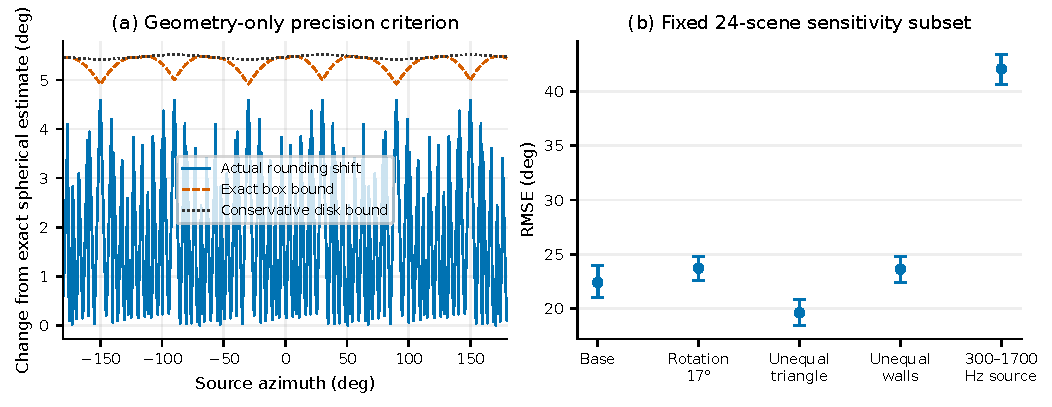
\includegraphics[width=\textwidth]{fig6_precision_sensitivity.pdf}
\caption{Precision and limited transfer checks. (a) Actual analytical rounding shift and deterministic bounds at 48 kHz, radius 0.05 m and source distance 1.5 m. The ordinate is relative to exact spherical-arrival estimates, not acoustic truth. (b) Five fixed sensitivity conditions; points are conditional RMSEs with record-bootstrap intervals. The source-band change retains a 300--3400 Hz estimator band.}
\label{fig:precision}
\end{figure*}

\section{Discussion}
The central practical result is that numerical and recording choices can alter the acoustic question being answered. Rounding continuous path arrivals creates an observable direct-path penalty. Starting with an empty source history produces an even larger apparent gain in an early reflected-field frame. A simulation that restarts the source for every short frame repeatedly samples this transient regime and cannot support a claim about continuous steady operation.

The appropriate control is paired propagation and source history at a fixed direct-referenced noise level, with independent numerical checks preceding interpretation. The direct-path and reflected-field rounding contrasts need not have the same sign: coherent interference and peak selection prevent simple addition of separate error magnitudes. Image coverage also matters; a nominal response duration without a sufficient image domain can omit influential paths. Reporting an achieved discrepancy at selected checks is more informative than only stating a large oversampling or image count.

The residual under averaging is conditional on the estimator and selected scenes. Longer averaging reduces random fluctuation but does not change the room transfer functions, finite-distance mismatch, or a stable preference for an incorrect correlation peak. Conversely, a finite residual at the longest tested duration is not proof of an infinite-time floor. The training/held-out split limits fitting to the same records used for evaluation; it does not convert three prescribed rooms into a representative population.

Several limitations constrain transfer. Ideal matched omnidirectional microphones avoid calibration, clock drift, gain mismatch, and platform artifacts. The source is synthetic band-limited Gaussian noise rather than speech or an operating machine. The room model is coherent, specular, and frequency-independent; real rooms may have different decay, scattering, and directional structure. The main source distance and array size are fixed, despite the broader analytical sweep. Rare peak switches can remain difficult to predict, and the numerical tolerance has been verified on specified controls and a fixed stochastic subset, not every possible signal.

Bootstrap intervals use only five independent records per short-record scene. They are useful conditional summaries, but their coverage has not been independently calibrated and the individual-scene intervals have limited empirical support. The balanced matrix and per-scene outputs make this limitation visible. The most useful release is therefore the complete computational record: configurations, input identities, exact method definitions, difficult outcomes, and reproducible figures. An external measured-room study would be an extension requiring new validation evidence, not a relabeling of the present numerical checks.

\section{Conclusion}
For the specified three-microphone model, arrival rounding and omitted source history produce distinct changes in estimated azimuth. Independent references and refinement keep the checked numerical discrepancy well below the principal interpreted effects. The matched startup experiment shows how a large apparent accuracy improvement can result from observing an unestablished reflected field. Held-out averaging reduces error but retains strong scene dependence. The geometry-only timing bound supplies a conservative analytical precision check with explicit limits; it does not certify noisy waveform localization. These results support careful simulation attribution and reproducibility rather than a universal acoustic error law.

\section*{Declarations and availability}
\textbf{Funding.} This work was self-funded by Aneesh Arnav Chikkala. The author reports no institutional affiliation.

\textbf{Conflicts of interest.} Author confirmation is pending for this review version. No absence-of-conflict declaration is inferred.

\textbf{Contributions and assistance.} A.A.C. selected the research direction and funded the work. Final scientific review and release approval remain pending. \mbox{OpenAI Codex} assisted substantively with planning, derivations, implementation, reference checks, literature synthesis, statistical analysis, figures, and manuscript drafting. The figures are deterministic plots generated with AI-authored code from retained results. The reference implementations and checks are internal computational verification; they are not external peer review. The assistance was not limited to language editing.

\textbf{Data and software.} The accompanying server-neutral reproducibility bundle contains per-frame results, configurations, source code, figure sources, environment records, verification reports, and reproduction instructions. No public repository or archive identifier has yet been assigned. Distribution licenses and public release await author decision. The supplement gives additional mathematical, statistical, and reproduction details. The local review package makes no claim of journal acceptance or editorial-policy eligibility.

\bibliographystyle{unsrtnat}
\begingroup\interlinepenalty=10000
\bibliography{references}
\endgroup
\end{document}
